The general equation of second degree is given by,
\begin{align}
ax^2 + 2bxy + cy^2 + 2dx +2ey +f = 0
\label{eq:solutions/13/7/2}
\end{align}
In vector from the equation \eqref{eq:solutions/13/7/2} can be expressed as,
\begin{align}
\vec{x}^T\vec{V}\vec{x} + 2\vec{u}^T\vec{x} + f = 0 
\label{eq:solutions/13/7/line_vec}
\end{align}
where,
\begin{align}
\vec{V} = \vec{V}^T = \myvec{a&b\\b&c}
\label{eq:solutions/13/7/3}
\end{align}
\begin{align}
\vec{u} = \myvec{d\\e}
\label{eq:solutions/13/7/4}
\end{align}
Now, comparing \eqref{eq:solutions/13/7/2} to \eqref{eq:solutions/13/7/1} we get, a =12, b=-5, c = 2, d = $\frac{11}{2}$,e = -$\frac{5}{2}$, f = k.  
Hence, substituting these values in \eqref{eq:solutions/13/7/3} and \eqref{eq:solutions/13/7/4} we get,
\begin{align}
\vec{V} = \myvec{12 & -5 \\ -5 & 2}
\end{align}
\begin{align}
\vec{u} = \myvec{\frac{11}{2} \\ -\frac{5}{2}}
\end{align}
\eqref{eq:solutions/13/7/1} represents pair of straight lines if,
\begin{align}
\mydet{\vec{V}&\vec{u}\\\vec{u}^T&f} = 0
\end{align}
\begin{align}
\mydet{12&-5&\frac{11}{2}\\-5&2&-\frac{5}{2}\\\frac{11}{2}&-\frac{5}{2}&k} = 0
\end{align}
\begin{align}
\implies k =2
\label{eq:solutions/13/7/5}
\end{align}
Lines Intercept if
\begin{align}
    |\vec{V}|<0\\
    |\vec{V}|=-1<0
\end{align}
Hence Line intercept.\\
Let $(\alpha,\beta)$ be their point of intersection, then
\begin{equation}\label{eq:solutions/13/7/eq6}
	\myvec{ a & b\\ b & c}\myvec{\alpha \\ \beta} = \myvec{-d \\ -e}
\end{equation}
Substituting in \eqref{eq:solutions/13/7/eq6}
\begin{align}
	\label{eq:solutions/13/7/eq11}\myvec{ 12 & -5\\-5 & 2}\myvec{\alpha \\ \beta} = \myvec{-\frac{11}{2} \\ \frac{5}{2}} \\
	\label{eq:solutions/13/7/eq12}\implies \myvec{\alpha \\ \beta} = \myvec{-\frac{3}{2} \\ -\frac{5}{2}}
\end{align}
Spectral Decomposition  of $\vec{V}$ is given as
\begin{equation}
\vec{V} = \vec{P}\vec{D}\vec{P}^T
\end{equation}
\begin{align}
	\label{eq:solutions/13/7/eq7}\vec{V} &= \myvec{ 12 & -5\\ -5 & 2}\\
	\label{eq:solutions/13/7/eq8}\vec{P} &= \myvec{-1-\sqrt{2} & -1 + \sqrt{2}\\ 1 & 1}\\
	\label{eq:solutions/13/7/eq9}\vec{D} &= \myvec{7 + 5\sqrt{2} & 0\\ 0 & 7 - 5\sqrt{2}}
\end{align}
Using Spectral decomposition concept and substution
\begin{align}
u_1(x-\alpha) + u_2(y-\beta) &= \pm \sqrt{-\frac{\lambda_2}{\lambda_1}}(v_1(x-\alpha) + v_2(y-\beta))\label{eq:solutions/13/7/eq10}
\end{align}
Substituting \eqref{eq:solutions/13/7/eq12}, \eqref{eq:solutions/13/7/eq8} and \eqref{eq:solutions/13/7/eq9} in \eqref{eq:solutions/13/7/eq10}
\begin{multline}\label{eq:solutions/13/7/eq13}
	\brak{-1-\sqrt{2}}\brak{x- \frac{-3}{2}} + \brak{y-\frac{-5}{2}} \\= \pm \sqrt{-\frac{7 +5\sqrt{2}} {7-5\sqrt{2}}}\brak{\brak{-1+\sqrt{2}}\brak{x- \frac{-3}{2}} + \brak{y-\frac{-5}{2}}}
\end{multline}
Simplifying \eqref{eq:solutions/13/7/eq13},
\begin{align}
	\label{eq:solutions/13/7/eq22}-6x + 2y - 4 = 0 \text{ and } -2x + y -\frac{1}{2} = 0\\
	\implies \brak{-6x + 2y - 4}\brak{-2x + y -\frac{1}{2}} = 0
\end{align}
Thus the equation of lines are
\begin{align}
\myvec{-6&2}\vec{x} = 4\\ 
\myvec{-2&1}\vec{x} = \frac{1}{2}
\end{align}
Hence, Plot is shown below 
\begin{figure}[ht!]
\centering
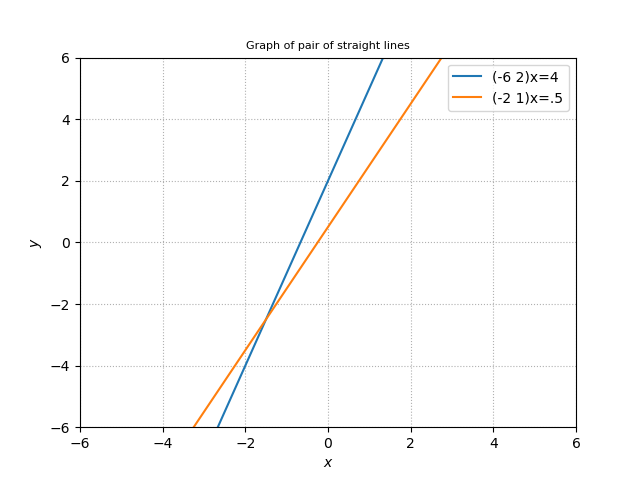
\includegraphics[width=\columnwidth]{./solutions/13/7/Figure.png}
\caption{Pair of lines}
\end{figure}
